\chapter{Operating System Concepts}

\section{Introduction}
A program that acts as an intermediary between a user application and the computer hardware.

\textbf{Operating system goals:}

\vspace{-0.5em}
\begin{itemize}[parsep=0.5em]
   \item Execute user programs and make solving user problems easier.
   \item Make the computer system convenient to use.
   \item Use the computer hardware in an efficient manner.
\end{itemize}

\section{System Structure}

\textbf{The components of a computer system:}

\begin{itemize}[parsep=0.5em]
   \item \textbf{Hardware:} provides basic computing resources CPU, memory, I/O devices.
   
   \item \textbf{Operating System:} controls and coordinates use of hardware among various applications and users.
   
   \item \textbf{Application Programs:} define the ways in which the system resources are used to solve the computing problems of the users. Example: word processors, compilers, web browsers, database systems, video games.
   
   \item \textbf{Users:} People, machines, other computers.
\end{itemize}

\begin{figure}[H]
    \centering
    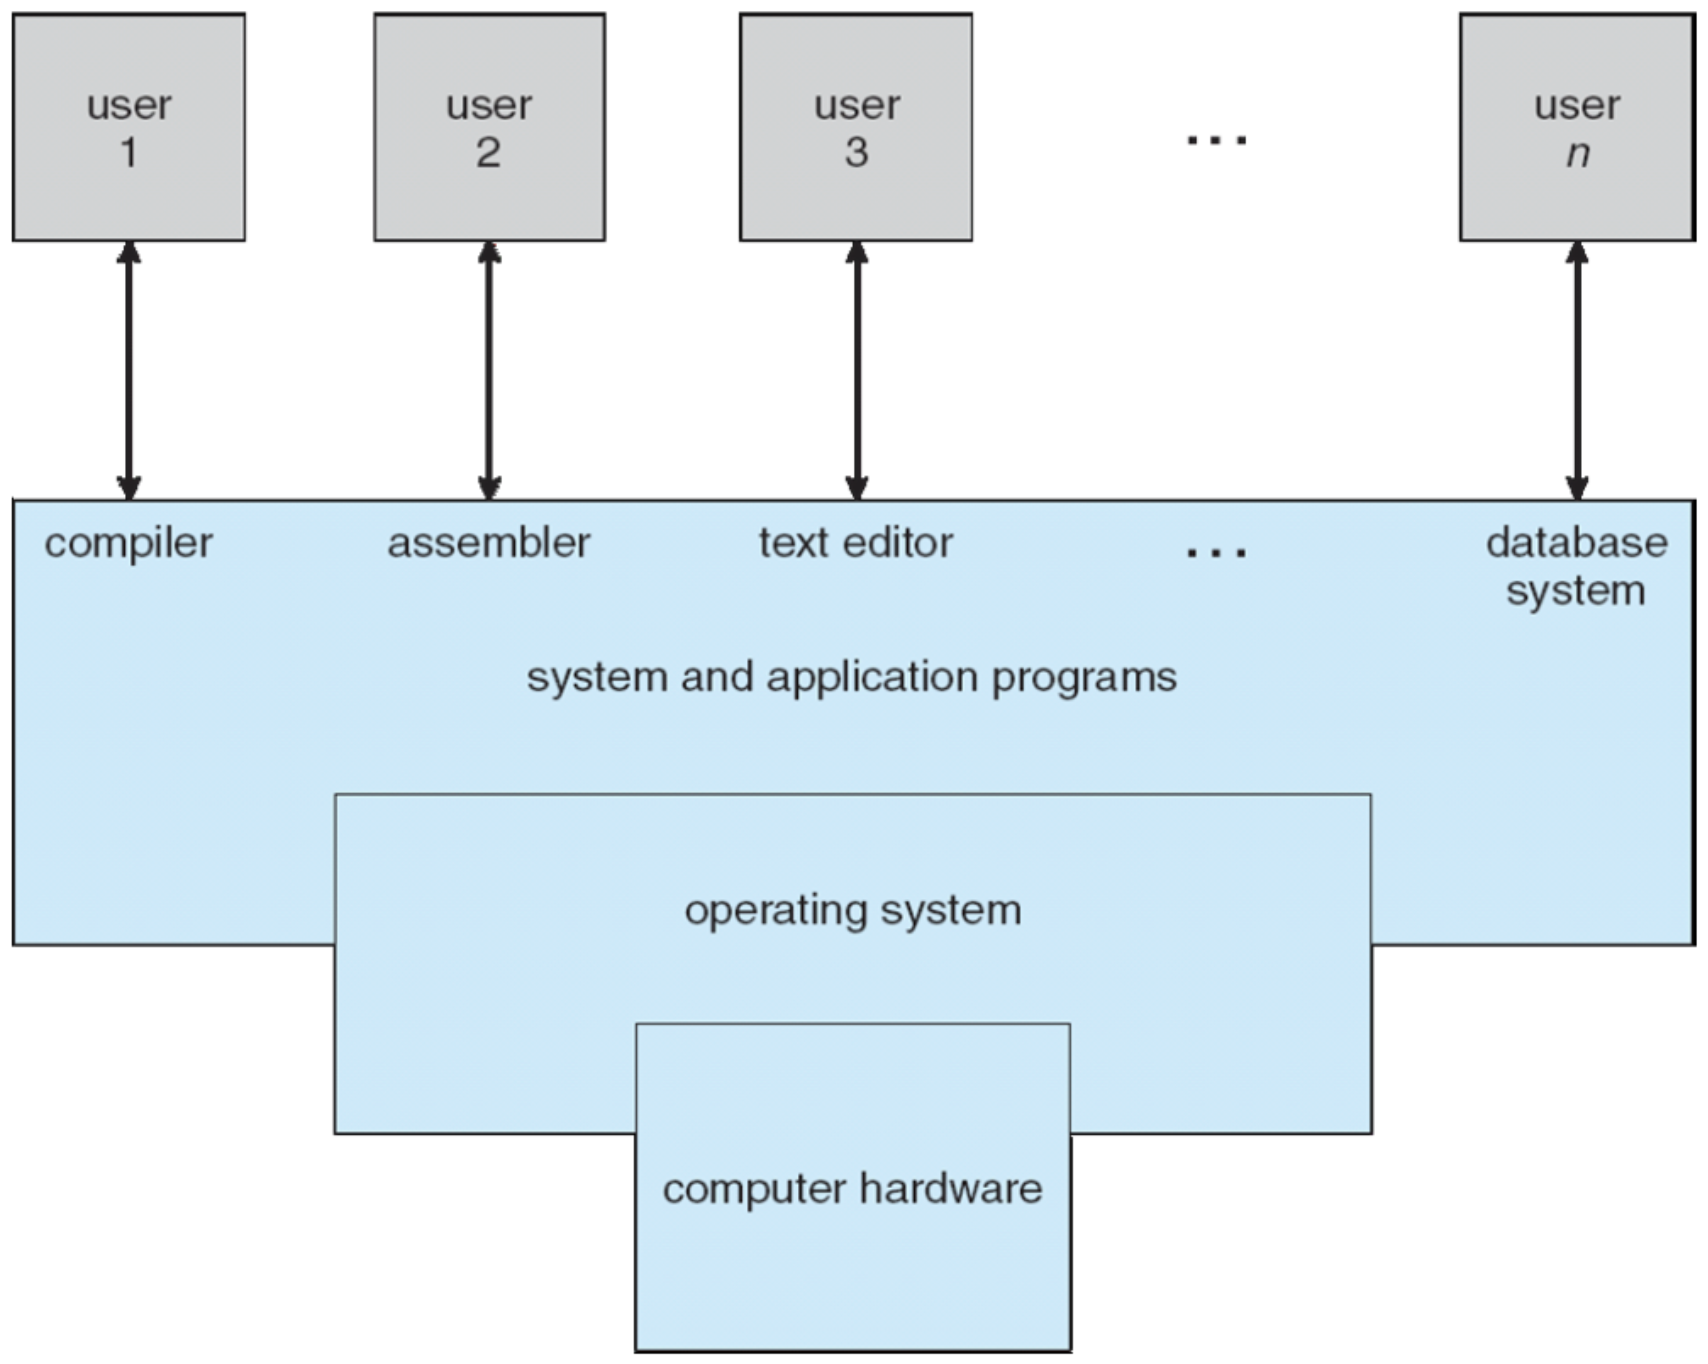
\includegraphics[width=0.45\textwidth]{figures/System Structure.png}
    \caption{Basic System Structure: Users, Application Programs, Operating System, and Hardware}
    \label{fig:system-structure}
\end{figure}


\section{Terminology}

\textbf{Kernel}: The kernel is a core component of an operating system that manages the system's resources and provides essential services for other software to run. It acts as a bridge between the hardware and software processes running on it.

\textbf{System Program}: A system program is a program that controls some aspect of the operation of a computer and is used to program the operating system software. Examples include: operating systems, networking systems, web servers, and data backup servers.

\textbf{System Call}: A system call is a mechanism that allows user-level applications to request services from the operating system's kernel. It provides an interface for programs to interact with the hardware and perform operations like file manipulation, process control, and communication.
\textit{Example includes:} \texttt{fork()}, \texttt{exec()}, \texttt{read()}, \texttt{write()}, \texttt{open()}, \texttt{close()}.

\textbf{Shell}: A shell is a program that provides a user interface to interact with the operating system, allowing users to execute commands or manage files and processes. It can be command-line based (like bash or cmd.exe) or graphical (like Windows Explorer or GNOME Shell).

\textbf{Program}: A program is a set of instructions written in a programming language that a computer can execute to perform a specific task or solve a problem. It can range from simple scripts to complex applications and typically runs under the control of an operating system.

\section{What Happens When We Run a Program?}

\begin{enumerate}[parsep=1em]
   \item A compiler translates high-level programs into an executable file.

   \begin{itemize}[parsep=0.5em]
      \item The executable contains CPU instructions and program data, each with specific memory addresses.
      \item Instructions are executed by the CPU, which implements an \textbf{Instruction Set Architecture (ISA)}.
      \item The CPU also contains a small set of registers, such as:
      \begin{itemize}
         \item \textbf{Program Counter (PC)}: points to the current instruction.
         \item \textbf{Registers}: for operands, memory addresses, and other purposes.
      \end{itemize}
   \end{itemize}

   \item When running an executable, the CPU performs the following steps:
   \begin{itemize}[parsep=0.5em]
      \item Fetches the instruction pointed to by the Program Counter (PC) from memory.
      \item Loads any data required by the instruction into registers.
      \item Decodes and executes the instruction.
      \item Stores the results back to memory if needed.
   \end{itemize}

   \item Most recently used instructions and data are in CPU caches for faster access.
\end{enumerate}


